\documentclass{article}
\usepackage{geometry}
\geometry{a4paper, margin=1in}
\usepackage[utf8]{inputenc}
\usepackage[T1]{fontenc}
\usepackage{lmodern}
\usepackage[english]{babel}
\usepackage{hyperref}
\usepackage{graphicx}
\begin{document}
	\title{Deep learning homework project: \ Waste classification}
	\author{Anna Gergály, Péter Mészáros}
	\maketitle
	
	\section{Introduction}
	Lot of waste. Waste management on this scale poses a lot of challenges and risks, both economically and environmentally. One of the best solutions we know at the moment besides trying to reduce the amount of waste created is to recycle. This helps recover resources and decreases chance of pollution and mitigates energy usage. 
	
	Despite it's obvious benefits it is not practiced at a large enough extent. The reasons for this mainly stem from the same issue: the need to separate the different materials. At home recycling often fails due to the cumbersome nature of the activity and in-facility waste separation is a very difficult task: manual classification is almost impossible due to sheer quantity and automatic waste sorting usually only works for certain materials in certain conditions.
	
	Our goal in this project was to create and review different solutions for a deep learning system that could provide automatic waste classification in such an environment.
	\section{Previous solutions}
	https://www.hindawi.com/journals/cin/2018/5060857/
	
	https://www.sciencedirect.com/science/article/pii/S2351978919307231
	
	https://towardsdatascience.com/advanced-waste-classification-with-machine-learning-6445bff1304f
	
	\section{Dataset}
	We assembled our dataset from 3 online sources (2 from Kaggle and 1 from Github) both to have a larger pool of images and a more varied one. There are pictures that contain the discarded item in front of plain backgrounds and ones that show them in a more organic way: dirty and/or muddy on a floor. 
	
	We settled on having eight categories within the datasets. These (glass, paper, cardboard, trash, metal, plastic, e-waste, medical) were selected mainly on two grounds: the available data and practical considerations. Most of these are well-known, already used recycling categories (glass, paper, cardboard, metal, plastic) and we have a multiple classes for non-recyclables, too. The main one of these is trash, but having extra categories for e-waste and medical waste makes sense as these are more dangerous environmentally and public health-wise. To make our datasets conform to these categorical standards we rearranged some of the pre-labeled data: e.g. merged different colored glasses and deleted categories we deemed unnecessary.
	
	The datasets together hold about 23,000 images which we decided to split in 14:3:3 ratio into training, validation and test sets.\ref{dataset} On the training set we decided to employ data augmentation: using the keras ImageDatasetGenerator we added zooming and shifting as well as both vertical and horizontal flips and 90° rotation to account for the fact that these items could be seen in any orientation in a waste management scenario.
	
	\begin{figure}
		\centering
		\resizebox{\textwidth}{!}{
			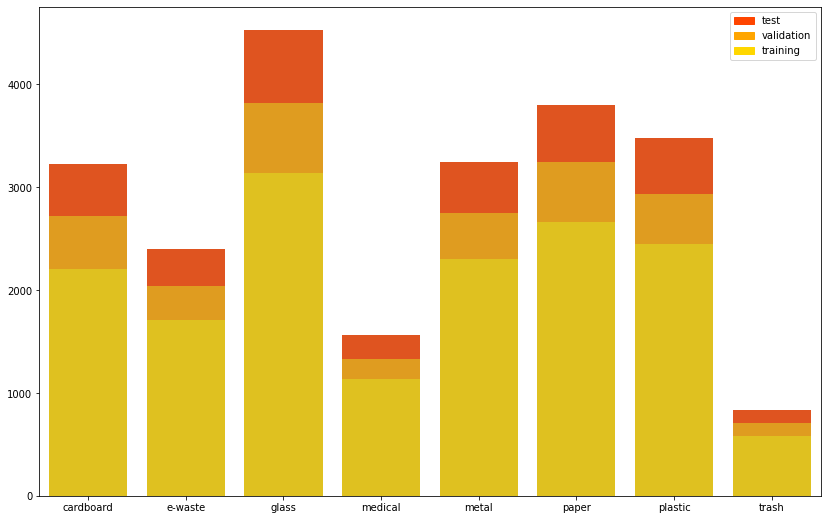
\includegraphics{dataset.png}}
		\caption{The size of the classes as divided into training, validation and test sets.}
		\label{dataset}
	\end{figure}
	
	\section{Proposed method}
	
	Our approach was to try out multiple pre-trained image classification CNNs by using transfer learning to prepare them for our specific task. The ones we use are EfficientNetB5 and MobileNetV2, both pre-trained on the imagenet dataset. To add a bit more interest and challenge to task we also decided to try our hands at building our own CNN from scratch.
	
	\subsection{EfficientNetB5}
	
	We chose the B5 variant of the EfficientNet because of it's moderate size and fairly strong results. We wanted something that would be feasible to train given our limited GPU-resources, but had a high-chance of yielding acceptable results. We removed the top-layer and substituted it with a few fit for our own needs: global average pooling, dropout and a dense layer with 8-nodes and a softmax activation to serve as an output layer in the 8-class classification problem.
	
	We trained this model, with only transfer learning using categorical crossentropy as our loss and categorical accuracy as our main metric, we used early stopping to stop the model from overfitting. The chosen batch size was 32, and 400 steps per epoch. We achieved a quite good result with this method (\textasciitilde$~87\% $ categorical accuracy) and we decided to go on with fine-tuning this model. 
	
	This however, was not possible, due to our technical limitations: the Google Colab environment could not support training this large of a model. This was one of the reasons we decided on a MobileNet for the third model: we wanted a transfer learning solution where we could also employ fine-tuning. 
	
	\subsection{Our own model}
	
	
	
	\subsection{MobileNetV2}
	
	
	
	\section{Evaluation method}
	
	\section{Results}
	
	\section{Discussion}
	
\end{document}